\documentclass[border=4pt]{standalone}
% Shared style for every diagram. Colour-blind-safe palette (Okabe-Ito).
\usepackage[T1]{fontenc}
\usepackage{helvet}
\renewcommand{\familydefault}{\sfdefault}
\usepackage{tikz}
\usetikzlibrary{arrows.meta,positioning,fit,backgrounds,calc,shapes.geometric,decorations.pathreplacing}
\definecolor{cblue}{HTML}{0072B2}
\definecolor{corange}{HTML}{E69F00}
\definecolor{cgreen}{HTML}{009E73}
\definecolor{cred}{HTML}{D55E00}
\definecolor{cpurple}{HTML}{CC79A7}
\definecolor{cgrey}{HTML}{6B7280}
\definecolor{csky}{HTML}{56B4E9}
\tikzset{
  >={Stealth[length=2.2mm]},
  box/.style={draw, rounded corners=3pt, align=center, minimum height=11mm, minimum width=22mm, font=\small, line width=0.7pt},
  real/.style={box, draw=cblue, fill=cblue!8},
  sim/.style={box, draw=corange, fill=corange!12},
  future/.style={box, draw=cgrey, dashed, fill=white},
  flow/.style={->, line width=0.8pt, draw=black!75},
  dflow/.style={->, line width=0.8pt, dashed, draw=cgrey},
  lbl/.style={font=\scriptsize, text=black!70},
  group/.style={draw=black!25, rounded corners=6pt, inner sep=6pt},
}

\begin{document}
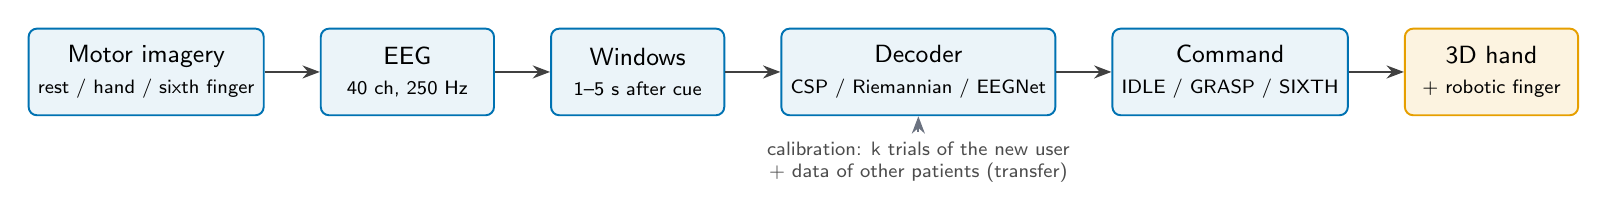
\begin{tikzpicture}[node distance=7mm]
  \node[real] (intent) {Motor imagery\\\scriptsize rest / hand / sixth finger};
  \node[real, right=of intent] (eeg) {EEG\\\scriptsize 40 ch, 250 Hz};
  \node[real, right=of eeg] (pre) {Windows\\\scriptsize 1--5 s after cue};
  \node[real, right=of pre] (dec) {Decoder\\\scriptsize CSP / Riemannian / EEGNet};
  \node[real, right=of dec] (cmd) {Command\\\scriptsize IDLE / GRASP / SIXTH};
  \node[sim, right=of cmd] (hand) {3D hand\\\scriptsize + robotic finger};
  \foreach \a/\b in {intent/eeg, eeg/pre, pre/dec, dec/cmd, cmd/hand} \draw[flow] (\a) -- (\b);
  \node[lbl, below=2mm of dec, align=center] (cal) {calibration: k trials of the new user\\+ data of other patients (transfer)};
  \draw[dflow] (cal) -- (dec);
\end{tikzpicture}
\end{document}
